


\chapter{State-space Covariates}
%\markboth{State-space Covariates}{}
\label{chapt.state-space}

\vspace{0.3cm}

Underlying all spatial capture recapture models is a point process
model describing the distribution of individual activity
centers (${\bf s}_i$) within the state space ($\cal{S}$). So far we have focused our
discussion on the homogeneous binomial point process,
${\bf s}_i \sim Uniform({\cal S}), i=1,2,\dots,N$, where $N$ is the
size of the population. This is a model of
``spatial-randomness''\footnote{The phrase ``complete
  spatial-randomness'' is reserved for the homogeneous Poisson point
  process}
because the intensity of the
activity centers is constant across the study area and the activity
centers are distributed independently of each other.

The spatial-randomness assumption is often viewed as restrictive
because ecological processes such as
territoriality and habitat selection can result in non-random
distributions of organisms. We have argued, however, that this
assumption is less restrictive than may be recognized because the
homogeneous point process actually allows for infinite
possible configurations of activity centers. Furthermore, given enough data,
the uniform prior will have very little influence on the estimated
locations of activity centers. Nonetheless, the homogeneous point
process model does not allow one to model population density using
covariates---a central objective of much ecological research.
For example, a homogeneous point process model
may result in a density surface map indicating that individuals were
more abundant in one habitat than another, but it does not do so
explicitly. A more direct approach would be to model density using
covariates as is done in generalized linear models (GLMs).% where a
%link function is used to connect the intensity parameter to the linear
%predictor. 

In this chapter we will present a method
for fitting inhomogeneous binomial point process models using
covariates in much the same way as is done with GLMs. The
covariates we consider differ
from those covered in previous chapters, which were typically
attributes of the animal ({\it e.g.} sex, age) and were used to model movement or encounter
rate. In contrast, here we wish to
model covariates that are defined for all points in the
the state-space, which we will refer to as
state-space, or density, covariates. These may
include continuous covariates such as elevation, or discrete
covariates such as habitat type.

\citet{borchers_efford:2008} were the first to propose an
inhomogeneous point process model for SCR models, and our approach is
similar to theirs with the exception that we will use a binomial
rather than a Poisson model because the binomial model is
easily integrated into our data augmentation scheme and is consistent
with the objective of determining how a {\it fixed} number of activity
centers are distributed with respect to covariates.

The method we use to accommodate inhomogeneous binomial point process
models within our MCMC algorithm is simple---we
replace the uniform prior with a prior describing the
distribution of
the $N$ activity centers conditional on the covariates. Development of
this prior, which does not have a
standard form, is a central component of this chapter.


\section{Homogeneous point process revisited}

The homogeneous Poisson point process is \emph{the} model of ``complete
spatial randomness'' and it is often used in ecology as a null model
to test for departures from randomness. Given its central role in the
analysis of point procesess, it is helpful to compare it with
the binomial model that we use in our SCR models. The
primary descriptor of the homogeneous point process model is the
``intensity'' parameter, $\mu$ which describles the expected number
of points in an infinitesimally small area. Thus the intensity
parameter can also be used to determine the expected number of points
in any region of the state-space $\cal{S}$. To denote this, we say
that the expected number of points in region $B \in \cal{S}$ is
$n(B) = A(B)\mu$ where $A(B)$ is the area of region $B$.  One property
of the Poisson model is that if we divide the entire state-space into
$k=1,\dots,K$ disjunct regions, the counts $\{n(B_k)\}$ are
independent and identically distributed, ({\it i.i.d.}). This is one
of the distinctions between the Poisson model and the binomial model,
for which the counts $n(B_k)$ are not {\it i.i.d.} as we will explain
shortly. This difference is also related to more important distinction
between the two models, namely that the binomial model
conditions on the number of points to be simulated $N$; whereas under
the Poisson model $N$ is random. Here is some simple R code to
illustrate this point.

\begin{verbatim}
mu <- 4                            # intensity
Np <- rpois(1, mu)                 # Np is random
PPP <- cbind(runif(Np), runif(Np)) # Poisson point process

Nb <- 4
BPP <- cbind(runif(Nb), runif(Nb)) # Binomial point process
\end{verbatim}

Note that in both models, the $N$ points are independent
of one another and distributed uniformly
throughout $\mathcal{S}$. Thus, the intensity at any point $x \in
\cal{S}$ is $\mu = 1 / A(\mathcal{S})$ where $A(\mathcal{S})$ denotes
the area of the state-space. For example, if the area of our
state-space is 4 km$^2$,
under a homogeneous model, the intensity is $\mu = 1/4$.

Although the Poisson model is typically described in terms of $\mu$,
the binomial model is not; rather, it
is more common to consider a discrete state space, such as a grid with
with $K$ pixels. Under the binomial model, the number of points in
each region is $n(B_k) \sim Bin(N, p_k)$
where $p_k = A(B)/A(\cal{S})$, ie $p_k$ is simply the fraction of
the state-space area in $B_k$. This discrete space representation of
the binomial point process is shown in Fig.~\ref{ch9:fig:homo}. The
state-space in this case is the unit square, and thus probability of a
point falling in each of the 25 disjunct regions is $p_k = 1/25$ and
thus the expected counts are simply $\mathbb{E}(n(B_k)) = Np_k$. In
the figure $N=50$ and thus we would expect 2 points per pixel, which
happens to be true in this case. Note also that these counts are not
independent realizations from a binomial distribution since $\sum_k
n(B_k) = N$. Instead, the model for the entire vector 
is ${\bf n(B)} \sim Multinomial(N, {\mathbf{\pi}} = (p_1, p_2, \dots,
p_K))$ \citep{illian:2008}. The dependence among counts has virtually
no practical consequence when the number of pixels is large. For
example, if we have 100 pixels, the number of counts in one pixels
tell you very little about the expected count in another
pixel. However, if there are only 2 pixels, then clearly the number of
points in one pixel tells you exactly how many will occur in the
remaining pixel. To gain familiarity with the multinomial distribution
and the discrete representation of space, use the \verb+rmultinom+
function in R to simulate counts similar to those shown in
Fig.~\ref{ch9:fig:homo}, for example using a command 
such as:

\begin{verbatim}
n.B_k <- rmultinom(1, size=50, probs=rep(1/25, 25))
matrix(n.B_k, 5, 5)
\end{verbatim}


\begin{figure}
\centering
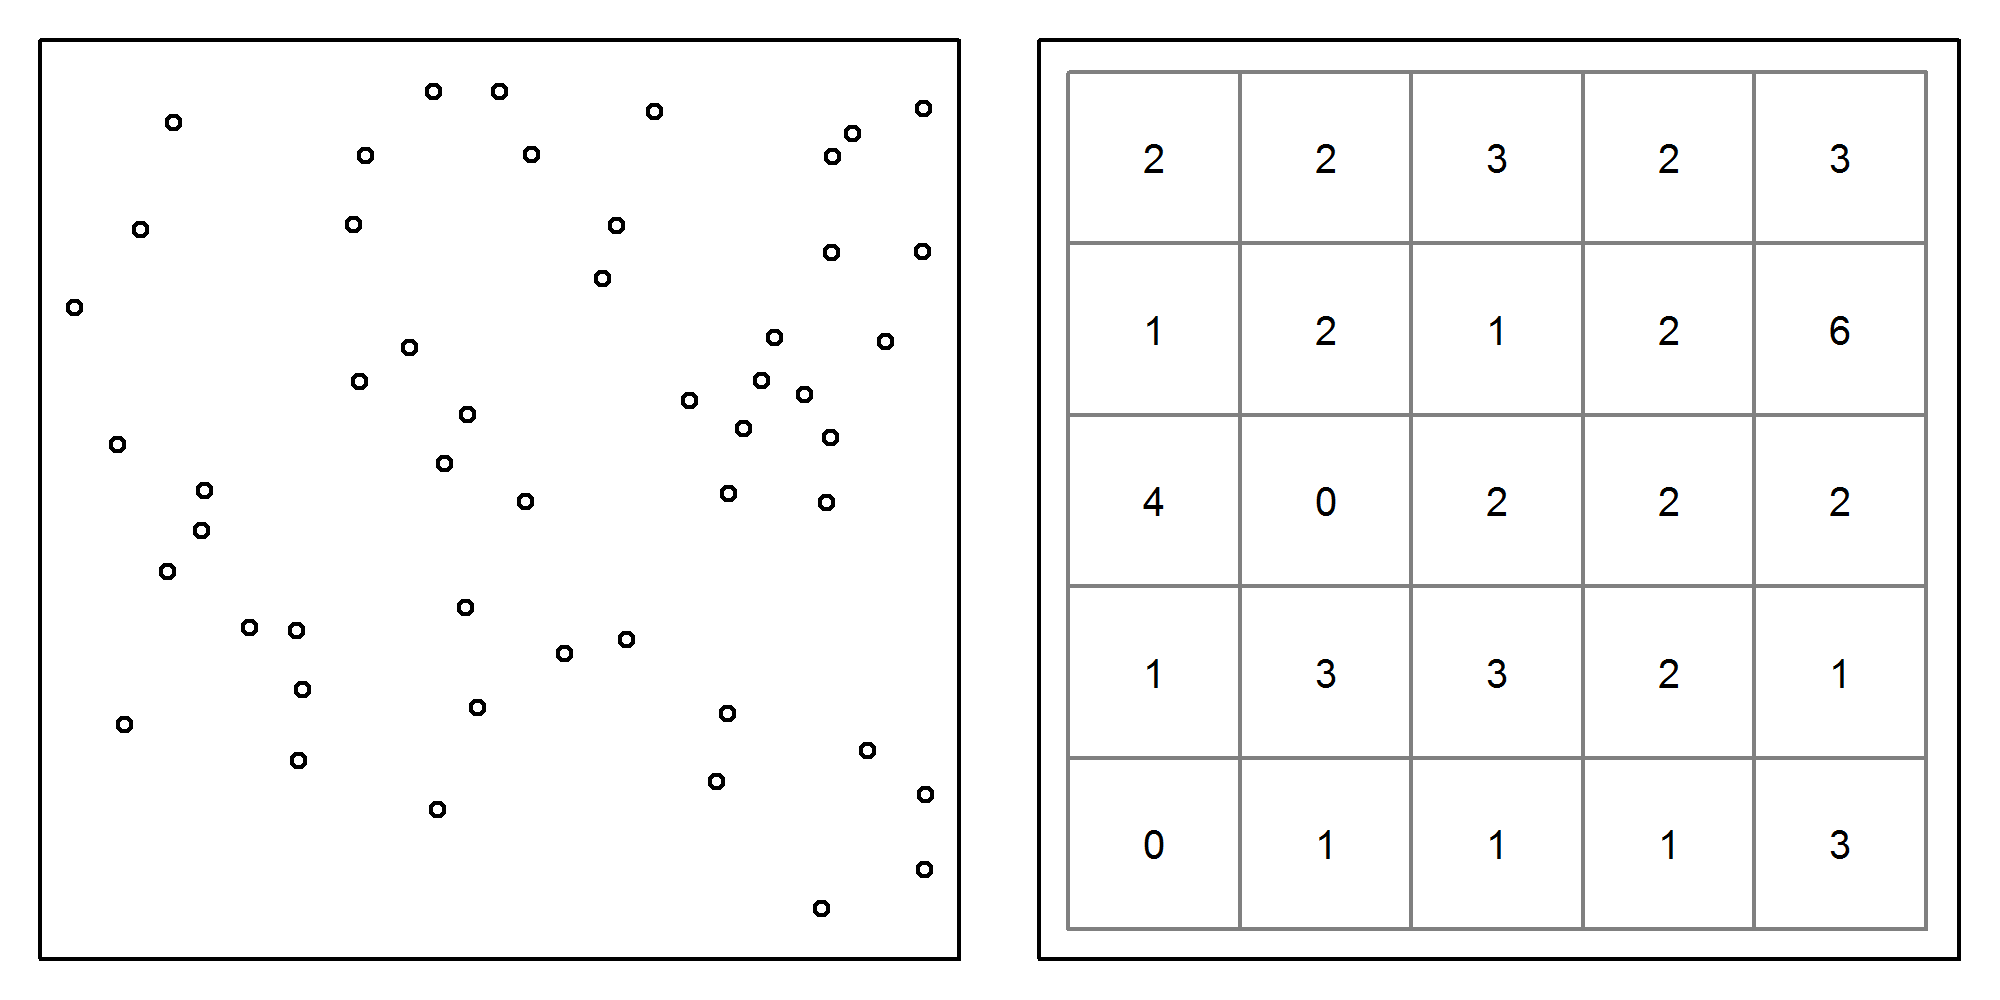
\includegraphics[width=5in,height=2.5in]{figs/homoPlots}
\label{ch9:fig:homo}
\caption{Homogeneous binomial point process with $N$=50 points
  represented in continuous and discrete space.}
\end{figure}


The discrete space representation of the binomial point process is of
practical importance when fitting SCR models because spatial covariates
are almost always represented in a discrete format, often called
``rasters'' in GIS-speak. In such cases, we often need to change our
definition of the prior for an activity center from $s_i \sim
Uniform(\cal{S})$ to $s_i \sim Multinomial(1, \mathbf{\pi})$. In the
latter case, the activity center is simply defined as an integer
representing pixel ``id''. Note also that the multinomial distribution
with an index of 1 (\emph{i.e.} \verb+size=1+ in \verb+rmultinom+) 
is referred to as the categorical distribution,  
which we will often make use of in the \verb+BUGS+ language.



\section{Inhomogeneous binomial point process}

As with the homogeneous model, the inhomogeneous binomial point process
model is developed conditional on $N$. The primary distinction is that
the uniform distribution is replaced with another distribution
allowing for the intensity parameter to vary spatially. To arrive at
this new distribution, define $\mu(x, {\bf \alpha})$ to be a function of
spatially-referenced covariates ($\mathbf{\alpha}$) available at all points of the state
space.  Subsequently we will drop the vector of cofficients from our
notation to be concise. Since an intensity must be strictly
positive, it is natural to model $\mu(x)$ using the log-link.
\[
\log(\mu(x)) = \sum_{j=1}^J \alpha_j v_j(x), \quad  x \in \cal{S}
\]
where $\alpha_j$ is the regression coefficient for covariate
$v_j(x)$. To be clear, $v(x)$ is the value of any covariate, such as
habitat type or elevation, at location $x$.  This equation should look
familiar because it is the standard linear model used in log-linear
GLMs. Note, however, that we have no need
for an intercept because it would be confounded with
$N$. This should be intuitive since an intercept would
represent the expected value of $N$ when $\alpha=0$, but we already
have a parameter in the model for expected abundance, namely $\mathbb{E}[N] =
\psi M$. Thus an intercept would be
redundant, and without it we are still able to achieve our goal of
describing the distribution of $N$ activity centers as a function of
spatial covariates.

Now that we have a model of the intensity parameter $\mu(x)$,
we need to develop the associated probability density function to use
in the place of the uniform prior used in the homogeneous
model. Remembering that
the integral of a pdf must be unity, we can create a pdf by dividing
$\mu(x)$ by a normalizing constant, which in this case is the integral
of $\mu(x)$ evlauated over the entire
state-space. The probability density function is therefore
\begin{equation}
f(x) = \frac{\mu(x)}{\int_{x \in \mathcal{S}} \mu(x)\, \mathrm{d}x}
\label{eq:pdf-ipp}
\end{equation}
Substituting this distribution for the
uniform prior allows us to fit inhomogeneous binomial point process
models to spatial capture-recapture data. We can also use this
distribution to obtain the expected number of individuals in any given
region. Specifically, the proprotion of $N$ expected to occur in any
region $B$ when heterogeneity in density is present is $p(B) = \int_B
f(x)\, \mathrm{d}x$. These are
also the multinomial cell probabilities if the regions are
disjoint and compose the entire state-space.

As a practical matter, note that the integral in the
demoninator of $f(x)$ is evaluated over space, and since we almost always regard as
space as two-dimensional, this is a two-dimensional integral that can
be approximated using the methods discussed in ref{ChXXX}. These methods include
Monte Carlo integration, Gaussian quadrature, etc... Alternatively, if
our state-space covariates are in raster format, \emph{i.e} they are
in discrete space, the integral can be replaced with a sum over
all pixels, which is much more efficient
computationally.

We now have all the tools needed to fit inhomogeneous point process
models. Before doing so, we note that this results in another point
process model for the 
observation process, $\lambda(x)$. As
a reminder, $\lambda(x)$ is the expected number of captures for a trap
at point $x$. As was true for the homogeneous model, this
intensity function is a convolution of the point process intensity
($\mu(x)$) and the encounter rate function,
$\lambda(x) = \mu(x) g(x,s)$.

In the next section we walk through a few examples, building up from
the simplest case where we actually observe the activity centers as
though they were data. In the second example, we fit our new model to simulated
data in which density is a function of a single continuous
covariate. In the last example, we model the intensity of activity
centers for a real dataset collected on jaguars (\emph{Panthera onca})
in Argentina +citep{some paper by Augustin}.

\section{Examples}

\subsection{Simulation and analysis of inhomogeneous point processes}

In SCR models, the point process is not directly observed, but in
other contexts it is. %the data in hand are the point locations
                      %themselves. 
Examples include the locations of disease
outbreaks or the locations of trees in a forest. Fitting inhomogeneous
point process models to such data is straight-forward and illustrates
the fundamental process that we will later embed in our MCMC algorithm
used to fit SCR models.

Suppose we knew the locations of 100 animals' activity
centers. To estimate the intensity surface $\mu(x)$ underlying these points, we
need to derive the likelihood for our data under this model. Given the
pdf $f(x)$, and assuming that the points are
mutually independent of one another, we may write
the likelihood as the product
of $R$ such terms, where $R=100$ is the sample size in this case,
\emph{ie} the observed number of activity centers.
\[
\mathcal{L}({\bf \alpha} | {\bf x}_i) = \prod_{i=1}^R f(x_i)
\]
Having defined the likelihood we could choose a prior and obtain the posterior for
$\bf \alpha$ using Bayesian methods, or we can find the maximum likelihood
estimates (MLEs) using standard numerical methods as is demonstrated
below.

First, let's simulate some data. Simulating data under an inhomogeneous point process model is often
accomplished using indirect methods such as rejection
sampling. Rejection sampling proceeds by
simulating data from a standard distribution and then accepting or
rejecting each sample using probabilities defined by the distribution
of interest. For more information, readers should consult an
accessible text like \citet{robert_casella:2004}. In our example, we
simulate from a uniform distribution and then accept or reject using
the (scaled) probability density function $f(x)$. Note that we first define a
spatial covariate (elevation) that is a simple function of the spatial
coordinates increasing from the southwest to the northeast of our
state-space.\footnote{Such functional forms of
covariates are rarely available, which is why continuous spatial
covariates are more often measured on a discrete grid.} 

The following R commands demonstrate the use of rejection sampling to
simulate an inhomogeneous point process for the covariate depicted in
Fig.~\ref{ch9:fig:elevMap}.


\begin{small}
\begin{verbatim}
# spatial covariate
# Elevation as a function of the coordinates at point x
elev.fn <- function(x) x[,1]+x[,2]

# 2-dimensional integration over [-1, 1] square
int2d <- function(alpha, delta=0.02) {
  z <- seq(-1+delta/2, 1-delta/2, delta)
  len <- length(z)
  cell.area <- delta*delta
  S <- cbind(rep(z, each=len), rep(z, times=len))
  sum(exp(alpha*elev.fn(S)) * cell.area)
  }

# Simulate PP using rejection sampling
set.seed(395)
N <- 100
count <- 1
s <- matrix(NA, N, 2) # matrix to hold simulated activity centers
alpha <- 2 # parameter of interest
Q <- max(c(exp(alpha*elev.min) / int2d(alpha),
           exp(alpha*elev.max) / int2d(alpha))) # Rejection sampling bound
while(count <= 100) {
  x.c <- runif(1, -1, 1); y.c <- runif(1, -1, 1) # proposed activity center
  s.cand <- cbind(x.c,y.c)
  elev.min <- elev.fn(cbind(-1,-1)); elev.max <- elev.fn(cbind(1,1))
  pr <- exp(alpha*elev.fn(s.cand)) / int2d(alpha)
  if(runif(1) < pr/Q) {
    s[count,] <- s.cand # accepted proposals
    count <- count+1
    }
  }
\end{verbatim}
\end{small}


\begin{figure}
\centering
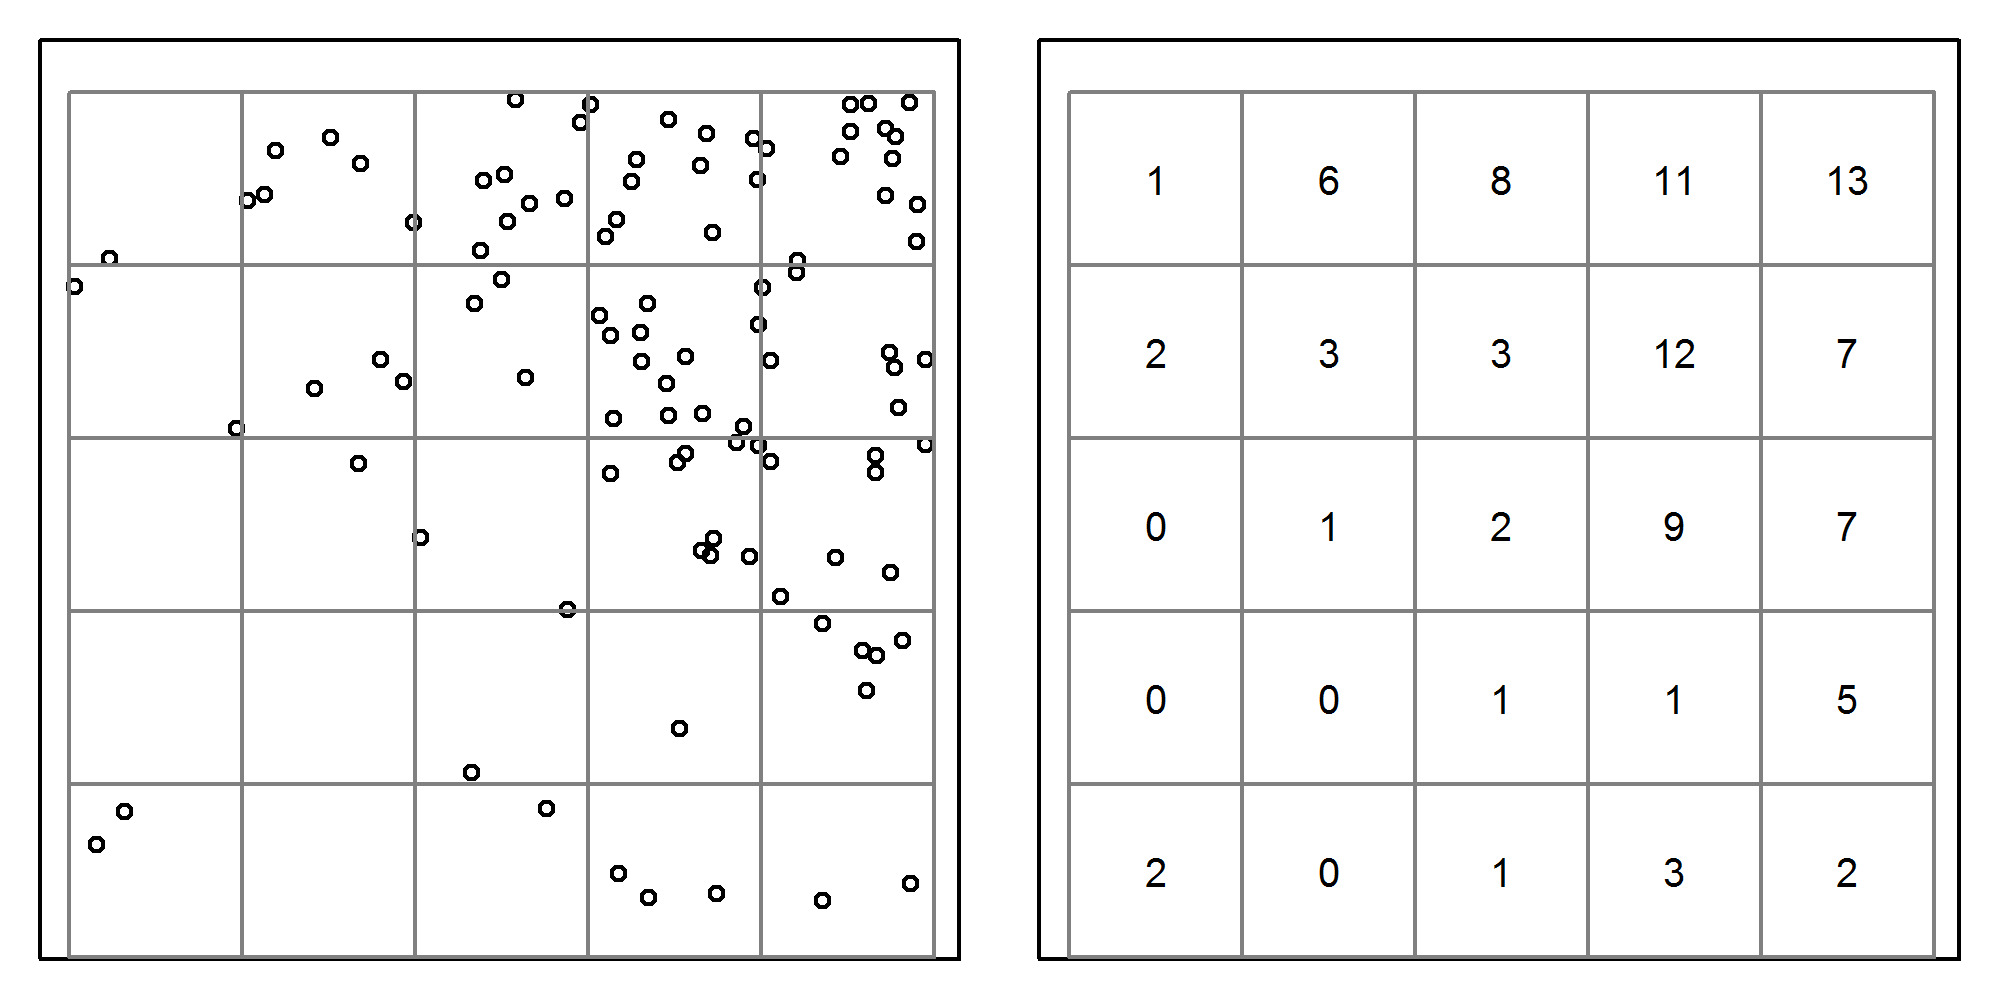
\includegraphics[width=5in,height=2.5in]{figs/heteroPlots}%{figs/elevMap}
\label{ch9:fig:elevMap}
\caption{An example of a spatial covariate, say elevation, and a
  realization of a inhomogeneous binomial point process with $N$=100
  and $\mu(x) = exp(\alpha Elev)$ where $\alpha=2$.}
\end{figure}

The simulated data are shown in Fig~\ref{fig:elevMap}. High elevations
are represented by light green and low elevations by dark green. The
activity centers of one hundred animals are shown as
points, and it is clear that these simulated animals prefer the high
elevations.  The underlying model describing this preference is
$\log(\mu(x)) = exp(\alpha \times Elevation(x))$
where $\alpha=2$ is the parameter to be estimated and $Elevation(x)$
is a function of the coordinates at $x$, as displayed on the map.

Given these points, we will now estimate $\alpha$ by minimizing the
negative-log-likelihood using \verb+R+'s \verb+optim+ function. 

\begin{small}
\begin{verbatim}
# Negative log-likelihood
nll <- function(beta) {
  -sum(beta*cov(S[,1], S[,2]) - log(int2d(beta)))
  }
starting.value <- 0
fm <- optim(starting.value, nll, method="Brent",
            lower=-5, upper=5, hessian=TRUE)
c(Est=fm$par, SE=sqrt(1/fm$hessian)) # estimates and SEs
\end{verbatim}
\end{small}


Maximizing the likelihood took a small fraction of a second, and we
obtained an estimate of $\hat{\alpha}=2.01$. Not bad! We could plug in
this estimate to our linear model at each point in the state-space to
obtain the MLE for the intensity surface.

This example demonstrates
that if we had the data we wish we had, {\it i.e.} if we knew the
coordinates of the activity centers, we could easily estimate the
parameters governing the underlying point process. Unfortunately, in
SCR models, the activity centers cannot be directly observed, but
spatial re-captures, that is captures of individuals at
multiple locations in space, provide us with the information needed to
estimate these latent parameters.

\subsection{Fitting inhomogeneous point process SCR model}

One of the nice things about hierarchical models is that they allow us
to break a problem up into a series of simple conditional
relationships. Thus,
we can simply add the methods described above into our existing MCMC
algorithm to simulate the posteriors of $\alpha$ conditional on the
simulated values of $\mathbf{s}_i$. To demonstrate, we will continue with
the previous example. Specifically, we will overlay a grid of
traps upon the map shown in Fig.~\ref{ch9:fig:elevMap}. We will then
simulate capture histories conditional upon the activity centers shown
on the map. Then, we will attempt to estimate the activity center
locations as though we did not know where they were.


Here is some \verb+R+ code to simulate the encounter histories under a
Poisson observation model, which would be appropriate if animals could
be detected multiple times at a trap during a single occassion. 

\begin{small}
\begin{verbatim}
# Create trap locations
xsp <- seq(-0.8, 0.8, by=0.2)
len <- length(xsp)
X <- cbind(rep(xsp, each=len), rep(xsp, times=len))

# Simulate capture histories, and augment the data
ntraps <- nrow(X)
T <- 5
y <- array(NA, c(N, ntraps, T))

nz <- 50 # augmentation
M <- nz+nrow(y)
yz <- array(0, c(M, ntraps, T))

sigma <- 0.1  # half-normal scale parameter
lam0 <- 0.5   # basal encounter rate
lam <- matrix(NA, N, ntraps)

set.seed(5588)
for(i in 1:N) {
    for(j in 1:ntraps) {
        distSq <- (s[i,1]-X[j,1])^2 + (s[i,2] - X[j,2])^2
        lam[i,j] <- exp(-distSq/(2*sigma^2)) * lam0
        y[i,j,] <- rpois(T, lam[i,j])
    }
}
yz[1:nrow(y),,] <- y # Fill
\end{verbatim}
\end{small}

Now that we have a simulated capture-recapture dataset $y$, and we have
augmented it to create the new data object $yz$, we are ready to
begin sampling from the posteriors. A commented Gibbs sampler written
in \verb+R+ is available online. There are two small parts of the
\verb+R+ code that distinguish it from previous code we have shown to
fit homogeneous point processes. First, we need to update the parameter
${\bf \alpha}$ conditional on all other parameters in the model. The code to
do so is: 

\begin{small}
\begin{verbatim}
D1 <- int2d(beta1, delta=.05)
beta1.cand <- rnorm(1, beta1, tune[3])
D1.cand <- int2d(beta1.cand, delta=0.05)
ll.beta1 <- sum(  beta1*cov(S[,1],S[,2]) - log(D1) )
ll.beta1.cand <- sum( beta1.cand*(S[,1]+S[,2]) - log(D1.cand) )
if(runif(1) < exp(ll.beta1.cand - ll.beta1) )  {
    beta1<-beta1.cand
}
\end{verbatim}
\end{small}

Next, we need to put the new prior on the activity centers:

\begin{small}
\begin{verbatim}
#ln(prior), denominator is constant
prior.S <- beta1*cov(S[i,1], S[i,2]) # - log(D1)
prior.S.cand <- beta1*(Scand[1] + Scand[2]) # - log(D1)
if(runif(1)< exp((ll.S.cand+prior.S.cand) - (ll.S+prior.S))) {
    S[i,] <- Scand
    lam <- lam.cand
    D[i,] <- dtmp
    }
\end{verbatim}
\end{small}

Applying this modified sampler to our data we obtain posterior
distributions summarized in Table~\ref{tab:simIPP}. Mixing is good, and as usual,
life is very nice when we are working with simulated data.



# MCCM code

source("thinSmcmc_exp.R")
ls()

fm1 <- scrIPP(yz, X, M, 3000, xlims=c(-1,1), ylims=c(-1,1),
            tune=c(0.002, 0.1, 0.25, 0.07) )

library(coda)
plot(mcmc(fm1$out))

rejectionRate(mcmc(fm1$out))






\begin{table}
\centering
\begin{tabular}{lccccc}
Parameter & Mean & SD  & q0.025 & q0.5 & q0.975 \\
\hline
$\alpha$    &&&&& \\
$\lambda_0$  &&&&& \\
$\sigma$    &&&&& \\
$N$        &&&&& \\
Density     &&&&& \\
\hline
\end{tabular}
\label{ch9:tab:simIPP}
\end{table}

It is worth noting that these models can also be fitted using
\verb+BUGS+ when the covariates are available in raster format. As
mentioned previously, we can define $s_i$ as the pixel id, and use the
categorical distribution as a prior.

\begin{verbatim} 
s[i] ~ dcat(probs[])
mu[i] <- exp(alpha*covariate[i])
probs[k] = mu[i]/sum(mu[])
\end{verbatim}

A good example of this is in +cite{Kery capricaillie}. One must be
aware, however, that for larger rasters, computing the denominator
will be a ghastly slow process when done 50,000 times in MCMC, but
this seems to run faster using \verb+JAGS+ than in \verb+BUGS+. 

[andy will have some stuff about this in Ch5]

Here is a cool example.


\subsection{The jaguar data}

Estimating density of large felines was difficult before the advent of
SCR. This is because you would never be able to conduct a distance
sampling analysis for such rare and cryptic species, and because
traditional capture-recapture methods don't yield estimates of
density, only population size within some unknown region. This example
not only demonstrates how readily density can be estimated for a
globally imperilled species, but it also shows the importance of
estimating density rather than just population size. 

[describe study]

A few aspects of this design are noteworthy. First, the dimensions and
configuration of the trap array differed among the regions of the trap
array. This fact alone could explain variation in the number of
animals exposed to sampling, which would have no biological
meaning. Furthermore, the area of inference is an irregular polygon
that was not sampled uniformly. Only by estimating density can we hope
to extrapolate our estiamates from the sampled region to get what we
are after. In this case, this is readily accomplished since the entire
state-space can be classified as one of the 3 levels of protection
from poaching. Of course, it general it is always preferable to sample
more uniformly throughout the area of interset in case some unmeasured
covariate biases the extrapolation.

To assess the influence of poaching on jaguar density, we considered 2
metrics of poaching pressure, one political and one continuous measure
of accessibility (Fig xxx). 



\section{MLE}

Maybe its easy to adapt the MLE code from chapter 5 for doing a
spatial covariate? For completeness it might be worth having that.

\section{Other ideas}

Should have some discussion on some ideas for building flexible
models. Might be cool to use the Ickstadt/Wolpert as a model for the
inhomogeneous point process. Dont have to do it, just mention it. Also
some kind of a spline model or similar.




\section{Summary}

When state-space covariates are available, we can model
density by replacing the uniform prior on the activity centers with a
prior based on a log-linear function of covariates.




